\documentclass[11pt]{article}

\usepackage[margin=1in]{geometry}
\usepackage{fancyhdr}
\usepackage{graphicx}
\pagestyle{fancy}
\usepackage{amsmath}
\usepackage{amssymb}
\usepackage[table]{xcolor}
\usepackage{booktabs}

\lhead{Homework 2}
\chead{Matthew Dees (30281707)}
\rhead{October 18, 2018}


\begin{document}

\begin{enumerate}
\item 
Conjugate-gradient implementation can be found in {\bf conjugate\_gradients.py}.

For the conjugate-gradient method I decided to use a stopping criteria similar to the one mentioned in the book. For evaluating the gradient output I used the formula $$|| \nabla f(\vec{x}) || \le \epsilon_{G}$$ where $ \epsilon_{G} = \epsilon_{abs} = 1.11 \times 10^{-14}$ (or it was varied as shown below). For evaluating the function output differential I used the following forumla as mentioned in the book $$ |f(\vec{x}_{k} + 1) - f(\vec{x}_{k})| \le \epsilon_{abs} + \epsilon_{R} | f(\vec{x_{k}}) | $$ where $\epsilon_{R} = \sqrt{\epsilon_{M}}$ where $\epsilon_{M} = 1.16 \times 10^{-16}$.
I used my 1D optimizer from homework 1 for the line search algorithm. I modified my algorithm such that it did not return a negative alpha. 

I used the following functions to test my algorithms:

$$ f(x) = (1 - x_0)^2 + 100(x_1 - x_0^2)^2 + 1 $$
$$ g(x) = x_0x_1 + (1-x_0)^2 + (2-x_1)^2+ (3-x_2)^2+ (4-x_3)^2+ (5-x_4)^2+ ... $$
$$ (6-x_5)^2+ (7-x_6)^2+ (8-x_7)^2+ (9-x_8)^2+ (10-x_9)^2 $$

I know my 10 dimensional function is not the most complicated, but hopefully it is good enough to show that my algorithm works in dimensions other than 2.
\\
For the output error I used the relative euclidean distance {\bf I felt that output function error was more useful to report than true function value because it is much easier to determine how close the optimizer was to the true value}:

$$ 100 \times \frac{Distance(\vec{X_{code}}, \vec{X_{optimum}})}{| \vec{X_{optimum}} |} $$
The mean of each table cell entry was calculated using:

$$\frac{1}{n} \sum_{i=1}^{n} x_{i}$$
\\
The standard deviation was calculated with the Bessel correction using the formula:

$$\sqrt{ \frac{1}{n - 1} \sum_{i = 1}^{n} (x_{i} - \bar{x})^2}$$

To gather enough data to calculate the mean and standard deviation I ran the optimizer 100 times using a starting vector where each point was drawn from the following Gaussian distribution (random.gauss(-10, 10)):

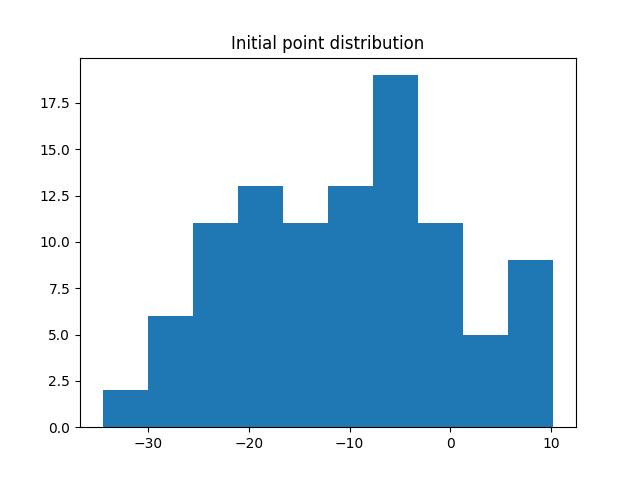
\includegraphics[width=6cm]{initial_point_dist.png}

The random restart frequency values were drawn from the following "uniform" distribution:

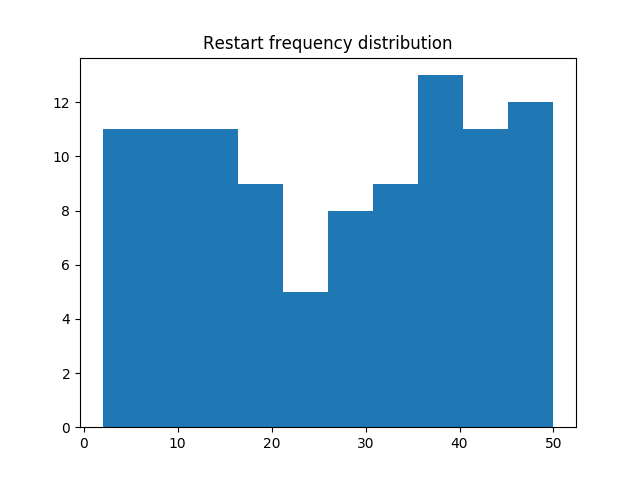
\includegraphics[width=6cm]{restart_frequency_dist.png}

The following algorithm was used to generate the varied epsilon (abs) values: Start at $ 1.0 \times 10^{-14} $ and end at $ 1.0 \times 10^{-5} $ multiplying by 10 each time.

I put a hard timeout limit of 15 seconds on both functions. If this value is hit the last calculated values are returned and a warning is produced.

{\bf Function 1}

$$ f(x) = (1 - x_0)^2 + 100(x_1 - x_0^2)^2 + 1 $$
Function 1 actual global minimum input vector = (1,1)

Function 1 evaluated at global minimum = 1.

The data from the runs can be found in files {\bf function1\_epsilon\_variation.pdf} and \\
{\bf function1\_gc\_freq\_variations.pdf}. The tables include mean and standard deviation for all of the requested parameter variations. From looking at the data it looks like the \%error increased for low restart frequency values (meaning the algorithm performed worse).  I saw on the discussion board that the TA recommended exploring all permutations of the variations (a1, a2, a3.. b1,b2... add a1,b1 a1,b2... etc to table) but I didn't like idea of changing two variables at a time because you cannot see how one variable change affects the algorithm. Perhaps we can discuss this in office hours. My epsilon variation results seemed counter intuitive because the \%error went down as my epsilon value went up. However, my iteration count went up as the epsilon value went down which seemed consistent with the algorithm (more iterations required for more precise answer). I also got a lot more variance as the epsilon value increased. I think this means that as the epsilon value is increased the variance of the starting initial point drastically affects the algorithm's performance on the Rosenbrock function. I also think the unintuitive \%error relationship can be attributed to the fact that I am comparing against the global minimum of (1, 1) which is hard for the algorithm to reach even with a good (low) epsilon, {\bf thus if it fins a wider variety of close-ish minimum that are within the valley the variance will be high.}

{\bf Function 2}

$$ g(x) = x_0x_1 + (1-x_0)^2 + (2-x_1)^2+ (3-x_2)^2+ (4-x_3)^2+ (5-x_4)^2+ ... $$
$$ (6-x_5)^2+ (7-x_6)^2+ (8-x_7)^2+ (9-x_8)^2+ (10-x_9)^2 $$

Function 2 actual global minimum input vector: [0, 2, 3, 4, 5, 6, 7, 8, 9, 10]

Function 2 evaluated at global minimum: 1

The data from the runs can be found in the tables in files  {\bf function2\_epsilon\_variation.pdf} and \\
{\bf function2\_gc\_freq\_variations.pdf}. My data for the restart frequency variations indicates that low frequency values (meaning the steepest descent step is taken more often) make the algorithm perform better for this function. I'm not really sure why this is and I think it will take more time than I have to figure it out. This is shown by the lower percent error for lower restart frequency values. The epsilon data also makes more sense for this function because as the epsilon value was increased the percent error and iterations both increased, as expected. With higher epsilon values the algorithm should run for a shorter amount of time and should be less accurate as it will stop earlier.

\item I implemented steepest descent in the file {\bf conjugate\_gradients.py}. The data for the runs can be found in {\bf steepest\_func1.pdf} and {\bf steepest\_func2.pdf}. The stopping criteria, mean calculation, and standard deviation calculation were the same as the conjugate-gradient test. Based on my data it looks like the steepest descent function performed worse for both functions. I was not expecting this to be the case because I expected the conjugate-gradient method to only offer an advantage for quadratic functions. I did run the conjugate-gradient method on some easier quadratic function at it vastly out performed the steepest descent method. I think the proper way to test would be to add a metric for computational cost to the steepest descent test since I believe it will take longer to execute, but I do not have time to do this since I was at CCS 2018 this week.

{\bf Conclusion}

I think it's safe to say the my implementation of conjugate-gradient is not good for the Rosenbrock function. I'm not sure if it is because I have a bug or not, since the other (easier) function I tested seem to work well. The data also has way more variance than I would have liked, but due to me not having a lot of time this week I had to limit the run count for each table row to 100. I think with a proper continuous integration setup with a dedicated server I would be able to run 10,000 times for each varied parameter and determine if the variance is due to an algorithm bug or the Rosenbrock function. It was fascinating to see the relationship between the GC iteration restart frequency and algorithm performance. It seems that low values for the frequency make the CG algorithm perfom worse for the Rosenbrock, but better for the 10D function. I think I would need to test on more functions to make a more general statement about the relationship between GC restart frequency and GC algorithm function performance for all functions. I'm still VERY confused as to why my variance is so high for the Rosenbrock function. Perhaps the determined minimum is highly dependent on the starting point because the valleys are so flat?
\end{enumerate}
\end{document}